\documentclass[aps,prb,groupedaddress,twocolumn,showpacs,dvipdfmx,superscriptaddress,pdftex]{revtex4-2}
\usepackage[whole]{bxcjkjatype}
\usepackage{amsmath}
\newcommand\numberthis{\addtocounter{equation}{1}\tag{\theequation}}
\usepackage{amssymb}
% \usepackage{bm}
% \usepackage{dcolumn}
% \usepackage{bm}
\usepackage{url}
% \usepackage{here}
% \usepackage{ulem}
\usepackage[caption=false]{subfig}
\usepackage[usenames,dvipsnames]{color}

\usepackage{graphicx}
\usepackage{booktabs}
\usepackage{rotating}
% \usepackage{makecell}
\usepackage{multirow}

\usepackage{fvextra}

% tiếng Việt
\usepackage[T5]{fontenc}
\usepackage[utf8]{inputenc}
\DeclareTextSymbolDefault{\DH}{T1}
%-------------------------------------
\newcommand{\tadd}[1]{\textcolor{red}{#1}}
\newcommand{\trem}[1]{{\color{red}\sout{#1}}}
\newcommand{\tcom}[1]{\textcolor{red}{\textbf{TI: #1}}}
\newcommand{\citehere}{\textcolor{red}{\textbf{(citation)}}}
\newcommand{\x}{\times}
%-------------------------------------
% \newcommand{\ghost}[1]{[#1]}
\newcommand{\ghost}[1]{}
%----------------------------------------
\def\red{\color{red}}
\def\blue{\color{blue}}
\def\green{\color{green}}
%%%%%%%%%%%%%%%%%%%%%%%%%%%%%%%%%%%%%%%%%
\begin{document}
\title{
    Meta-learning in movement prediction problem of aperiodic time-series data
}
%%%%%%%%%%%%%%%%%%%%%%%%%%%%%%%%%%%%%%%%%
\author{Bao-Long Nguyen}
\email{mwklng2309@icloud.com}
\affiliation{School of Information Science, JAIST, Ishikawa, Japan}
%
\author{Tom Ichibha}
\email{ichibha@icloud.com}
\affiliation{School of Information Science, JAIST, Ishikawa, Japan}
%
\author{Kenta Hongo}
\email{kenta_hongo@mac.com}
\affiliation{Research Center for Advanced Computing Infrastructure, JAIST, Ishikawa, Japan}
%
\author{Ryo Maezono}
\email{rmaezono@mac.com}
\affiliation{School of Information Science, JAIST, Ishikawa, Japan}
%
\date{\today}
%%%%%%%%%%%%%%%%%%%%%%%%%%%%%%%%%%%%%%%%%
\begin{abstract}

    \textbf{Abstract}. Predicting aperiodic time-series data (e.g. stock price, foreign exchange, Bitcoin price,...) is a difficult task for machine learning models because this type of data has high variance and is not stationary; does not show clear cycles, making it difficult to extract features; depends not only on past values but also on external factors, which make them unstable and non-cyclical such as economic and political situations. To overcome the above challenges, we use Meta-learning to train a combined \verb|LSTM| and \verb|CNN| network, thereby effectively extracting and synthesizing hidden features of the data over time. Experiments on foreign exchange data of 60 currency pairs over 24 years (2000-2024) show that the proposed method performs well and has higher accuracy than the \verb|NHITS| - the state-of-the-art model in 2023 on time-series data, in the task of predicting the trend (upward or downward) of the next trading day.

    % Dự đoán aperiodic time-series data (e.g. stock price, foreign exchange, Bitcoin price,...) là một tác vụ khó khăn đối với các mô hình học máy bởi vì loại dữ liệu này có phương sai cao và không cố định; không thể hiện chu kỳ rõ ràng nên khó rút trích đặc trưng; không chỉ phụ thuộc vào giá trị quá khứ mà còn phụ thuộc các yếu tố ngoại lai, điều khiến chúng bất ổn và không có chu kỳ như tình hình kinh tế, chính trị. Để khắc phục các thách thức nêu trên, chúng tôi sử dụng Meta-learning để huấn luyện kết hợp mạng \verb|LSTM| và \verb|CNN|, từ đó rút trích và tổng hợp hiệu quả các đặc trưng ẩn của dữ liệu theo thời gian. Thực nghiệm trên dữ liệu foreign exchange của 15 cặp tiền tệ trong vòng 24 năm (2000-2024) cho thấy phương pháp đề xuất hoạt động tốt và có độ chính xác cao hơn mô hình \verb|NHITS| - state-of-the-art model của năm 2023 trên dữ liệu time-series, trong bài toán dự đoán xu hướng (upward or downward) của ngày giao dịch tiếp theo.
\end{abstract}
%----------------------------------------
\keywords{Meta-learning, \verb|LSTM|, \verb|CNN|, Aperiodic time-series data, Foreign exchange}
\maketitle

%%%%%%%%%%%%%%%%%%%%%%%%%%%%%%%%%%%%%%%%%
\section{Introduction}
\label{sec.intro}
%%%%%%%%%%%%%%%%%%%%%%%%%%%%%%%%%%%%%%%%%

% Aperiodic time-series prediction nói chung hay foreign exchange (FX) prediction nói riêng từ lâu đã là vấn đề đáng quan tâm của nhiều nghiên cứu \citep{li2019multi, islam2021foreign, heryadi2021foreign}. Hai kỹ thuật chính được sử dụng trong aperiodic time-series prediction là fundamental analysis and technical analysis \cite{ayitey2023forex}. Trong khi fundamental analysis thiên về phân tích các yếu tố tác động từ bên ngoài và khó có thể capture từ các biến thiên giá trị trong quá khứ như chính sách, chiến lược kinh tế của công ty, quốc gia để dự đoán tương lai; technical analysis dựa hoàn toàn vào lịch sử biến động giá trị để phân tích xu hướng tương lai.

Aperiodic time-series prediction in general or foreign exchange (FX) prediction in particular has long been a matter of concern for many researchers \citep{li2019multi, islam2021foreign, heryadi2021foreign}. The two main techniques used in aperiodic time-series prediction are fundamental analysis and technical analysis \cite{ayitey2023forex}. While fundamental analysis focuses on analyzing external factors, which are difficult to be captured from past value fluctuations such as policies and economic strategies of companies and countries to predict the future; technical analysis relies entirely on historical value fluctuations to analyze future trends.

\vspace{2mm}

% Việc dự đoán trên aperiodic time-series data gặp một vài thách thức cố hữu. Trong đó có thể kể tới: (1) - Variance của loại dữ liệu này biến thiên mạnh qua các thời kỳ. Từ đó giả thuyết rằng chúng tuân theo một phân phối để có thể xấp xỉ lỗi là không thể sử dụng được, dẫn đến việc các mô hình học máy khó có thể dự đoán chính xác giá trị cũng như xu hướng trong tương lai; (2) - Aperiodic data không tuân theo bất kỳ quy luật rõ ràng nào nên việc học các đặc trưng ẩn của dữ liệu để tiến hành dự đoán gặp rất nhiều khó khăn; (3) - Aperiodic time-series data (e.g. giá cổ phiếu của một công ty) không hoàn toàn phụ thuộc vào dữ liệu quá khứ mà còn phụ thuộc nhiều yếu tố ngoại lai (e.g. tin tức, tình hình kinh tế, chính trị) \cite{li2019multi}.

Predicting on aperiodic time-series data faces several inherent challenges: (1) - The variance of this type of data varies greatly over time. Therefore, the assumption that they follow a distribution to approximate the error cannot be used, leading to machine learning models having difficulty accurately predicting future values and trends; (2) - Aperiodic data does not follow any explicit rules, so learning the hidden features of the data to make predictions is very difficult; (3) - Aperiodic time-series data (e.g. a company's stock price) depends not only on past data but also on many external factors (e.g. news, economic situation, politics) \cite{li2019multi}.

\vspace{2mm}

% Đối với thách thức đầu tiên, các mô hình ensemble [cite something here] thường được sử dụng để hạn chế ảnh hưởng của sự biến đổi variance. Ensemble model giúp cung cấp một cái nhìn tổng quát, tổng hợp từ nhiều khía cạnh dựa trên các sub-models, từ đó giúp mô hình tổng quát thích ứng được với sự thay đổi mạnh của variance. Chúng tôi tiếp cận bài toán theo hướng này nhưng ở mức cao hơn bằng cách sử dụng Meta-learning (ML) \cite{finn2017model}. Phương pháp này tổng hợp hiệu quả tham số của các mô hình cục bộ, giúp giảm thiểu đáng kể variance loss.

For the first challenge, ensemble models [cite something here] are often used to mitigate the effects of variance variation. Ensemble models provide a holistic, multi-perspective view based on sub-models, thereby helping the overall model adapt to strong variance changes. We approach the problem in a similar but higher-level way using Meta-learning (ML) \cite{finn2017model}. This method effectively aggregates the parameters of local models, which helps to significantly reduce variance loss.

\vspace{2mm}

% Để khắc phục thách thức thứ hai, các nghiên cứu phần lớn sử dụng các đặc trưng rút trích được từ Long short-term memory neural network (\verb|LSTM|) \cite{hochreiter1997long}, Artificial neural network (\verb|ANN|), và Convolution neural network (\verb|CNN|) \cite{lecun1989handwritten}. Cụ thể, trong năm 2022, 20\% tổng số các bài báo liên quan đến dự đoán chỉ số tài chính sử dụng \verb|LSTM|, 20\% sử dụng \verb|ANN| và 6\% sử dụng \verb|CNN| \cite{ayitey2023forex}. Để tận dụng hết được các đặc trưng được rút trích bởi các mô hình nêu trên, chúng tôi đề xuất phương pháp kết hợp các đặc trưng này.

To overcome the second challenge, most studies use features extracted from Long short-term memory neural network (\verb|LSTM|) \cite{hochreiter1997long}, Artificial neural network (\verb|ANN|), and Convolution neural network (\verb|CNN|) \cite{lecun1989handwritten}. Specifically, in 2022, 20\% of all publications related to financial index prediction used \verb|LSTM|, 20\% used \verb|ANN|, and 6\% used \verb|CNN| \cite{ayitey2023forex}. To make full use of the features extracted by the above models, we propose a method that combines these features.

\vspace{2mm}

% Đối với thách thức thứ ba, nghiên cứu \cite{fama1970efficient} đưa ra giả thuyết rằng các time-series datasets khác nhau của cùng một lĩnh vực tại cùng thời điểm phản ánh sự tác động của các yếu tố ngoại lai. Ví dụ, các nghiên cứu \citep{overreactioncontrarian, mech1993portfolio} cũng chỉ ra sự phụ thuộc giữa chỉ số tài chính của một công ty nhất định và các chỉ số của các công ty khác. Điều này càng làm tăng tính đúng đắn của giả thuyết trong nghiên cứu \cite{fama1970efficient}. Ngoài ra, chúng tôi cho rằng, loại dữ liệu này còn có những phụ thuộc ngầm vào các thời điểm nhất định trong quá khứ (hidden long-term dependency). Đối với cách tiếp cận truyền thống, người ta sử dụng một lượng dữ liệu quá khứ cố định (lookback window) để huấn luyện mô hình. Điều này gây một trở ngại lớn cho quá trình học vì các đặc trưng dài hạn theo thời gian sẽ bị quên. Mặt khác, ML chia nhỏ tập dữ liệu thành nhiều phần để học và tổng hợp hiệu quả các tham số học được nên có thể xử lý tốt thách thức này.

Regarding the third challenge, \cite{fama1970efficient} research hypothesizes that different time-series datasets of the same domain at the same time point reflect the impact of extraneous factors. For example, studies \citep{overreactioncontrarian, mech1993portfolio} show the dependence between the financial ratios of a given company and the ratios of other companies. This further strengthens the hypothesis in study \cite{fama1970efficient}. In addition, we argue that this type of data also has hidden long-term dependencies. For the traditional approach, people use a fixed amount of past data (lookback window) to train the model. This causes a big obstacle to the learning process because long-term features over time will be forgotten. On the other hand, ML divides the dataset into many parts to learn and synthesize the learned parameters effectively, so it can handle this challenge well.

\vspace{2mm}

% Cuối cùng, chúng tôi chứng minh tính ưu việt của thuật toán đề xuất bằng cách giải bài toán dự đoán xu hướng (tăng hoặc giảm) của tỉ giá ngoại hối và so sánh kết quả với mô hình SOTA hiện tại (\verb|NHITS| \cite{challu2023nhits}) trên hai loại dữ liệu: (1) - Dữ liệu tỉ giả của cặp tiền tệ USD/JPY; (2) - Dữ liệu tỷ giá của 60 cặp tiền tệ, cấu thành từ 18 quốc gia. Các tập dữ liệu này được công khai trên Internet và có thể tải về dễ dàng. Bản cài đặt chính thức có thể xem tại [bỏ cái link github vào đây].

Finally, we demonstrate the superiority of the proposed algorithm by solving the problem of predicting the trend (up or down) of foreign exchange rates and comparing the results with the existing state-of-the-art (SOTA) model (\verb|NHITS| \cite{challu2023nhits}) on two types of data: (1) - USD/JPY exchange rate data; (2) - Exchange rate data of 60 currency pairs, comprising 18 countries. These data sets are publicly available on the Internet and can be easily downloaded. The official implementation can be found at [insert github link here].

\vspace{2mm}

In summary, our main contributions are as follows:

\begin{itemize}
    % \item Kết hợp đặc trưng: Rút trích đặc trưng bằng cách kết hợp các đặc trưng của \verb|LSTM| và \verb|CNN|.
    \item Feature combination: Extract feature using \verb|LSTM| and \verb|CNN| and combine them.

    % \item Hidden long-term dependency: Chứng minh thực nghiệm rằng một aperiodic time-series data nhất định không chỉ phụ thuộc vào các yếu tố ngoại lai mà còn có các phụ thuộc ẩn với chính nó tại nhiều thời điểm khác nhau trong quá khứ.
    \item Hidden long-term dependency: Experimentally demonstrate that a given aperiodic time-series data not only depends on external factors but also has hidden dependencies with itself at various points in the past.

    % \item Tổng hợp hiệu quả tham số mô hình: Sử dụng ML thay cho các mô hình ensemble truyền thống trong việc tổng hợp kết quả từ các mô hình học máy.
    \item Efficient model parameter aggregation: Use ML instead of traditional ensemble models to aggregate results from machine learning models.

    % \item Experiment: Thực nghiệm trên các bộ dữ liệu về tỉ giá hối đoái và so sánh với mô hình SOTA \verb|NHITS| để chứng minh tính hiệu quả của phương pháp đề xuất.
    \item Experiment: Experiment on exchange rate datasets and compare with \verb|NHITS| - the SOTA model to demonstrate the effectiveness of the proposed method.
\end{itemize}

%%%%%%%%%%%%%%%%%%%%%%%%%%%%%%%%%%%%%%%%%%%%%%%%%%%%
\section{Related work}
\label{sec.relatedWork}
%%%%%%%%%%%%%%%%%%%%%%%%%%%%%%%%%%%%%%%%%%%%%%%%%%%%

\subsection{LSTM \& CNN model}

% Như đã đề cập, \verb|LSTM| là mạng neural rất phổ biến trong việc handle các bài toán liên quan đến dự đoán trên dữ liệu time-series. \verb|LSTM| được sử dụng phổ biến như vậy bởi vì nó xử lý tốt vấn đề vanishing gradient (dễ dàng bắt gặp khi sử dụng Recurrent neural network) và có thể khai thác hiệu quả các mối quan hệ phi tuyến trong dữ liệu. Thật vậy, bằng cách duy trì cell-state trong mỗi iteration, \verb|LSTM| có thể khắc phục vấn đề vanishing gradient, từ đó bảo toàn khả năng capture các phụ thuộc dài hạn \cite{cheng2018applied}. Ngoài ra, \verb|LSTM| thực hiện rút trích đặc trưng với các hàm kích hoạt phi tuyến, giúp các tham số mô hình có thể capture tính phi tuyến của dữ liệu \cite{he2016exploiting}. Hai yếu tố nêu trên khiến cho \verb|LSTM| trở thành lựa chọn đầu tiên được nghĩ đến khi giải quyết các bài toán trên dữ liệu time-series.

As aforementioned, \verb|LSTM| is a well-known neural network for handling prediction problems on time-series data. \verb|LSTM| is commonly used because it handles the problem of vanishing gradients well (easily encountered when using Recurrent neural networks) and can effectively exploit nonlinear relationships in data. Indeed, by maintaining the cell-state in each iteration, \verb|LSTM| can overcome the vanishing gradient problem, thereby preserving the ability to capture long-term dependencies \cite{cheng2018applied}. In addition, \verb|LSTM| performs feature extraction with nonlinear activation functions, which helps the model parameters capture the nonlinearity of the data \cite{he2016exploiting}. These factors make \verb|LSTM| to be the first choice to think of when solving problems on time-series data.

\vspace{2mm}

% Mạng \verb|CNN| được sử dụng rất nhiều trong các tác vụ xử lý hình ảnh \citep{naranjo2020review, sharma2018analysis} bởi khả năng tổng hợp các quan hệ cục bộ. Không chỉ vậy, \verb|CNN| còn được dùng rất nhiều trong các tác vụ xử lý dữ liệu time-series như speech recognition \cite{dua2022developing}, natural language processing \cite{varshitha2023natural}. Điều đó chứng tỏ được khả năng của \verb|CNN| trong việc khám phá mối quan hệ thời gian cục bộ giữa các mẫu dữ liệu. Mặc dù vậy, \verb|CNN| lại rất ít được dùng trong các tác vụ dự đoán stock price hay foreign exchange. Trong nghiên cứu này, chúng tôi tận dụng khả năng rút trích đặc trưng cục bộ tuyệt vời của \verb|CNN| để tích hợp thêm thông tin ẩn vào quá trình huấn luyện của mô hình.

\verb|CNN| is widely used in image processing tasks \citep{naranjo2020review, sharma2018analysis} because of its ability to synthesize local relationships. Not only that, \verb|CNN| is also widely used in time-series data processing tasks such as speech recognition \cite{dua2022developing}, natural language processing \cite{varshitha2023natural}. This proves the ability of \verb|CNN| in discovering local temporal relationships between data samples. However, \verb|CNN| is rarely used in aperiodic time-series data prediction tasks. In this study, we take advantage of \verb|CNN|'s excellent local feature extraction ability to incorporate more hidden information into the model training process.

\subsection{Model-agnostic Meta-learning (MAML)}

% Các thuật toán Meta-learning (ML), điển hình là MAML \cite{finn2017model} được biết đến với khả năng huấn luyện một mô hình có tính tổng quát cao, thích ứng nhanh trên tập dữ liệu mới thông qua một lượng nhỏ dữ liệu và số bước huấn luyện \citep{hospedales2021meta, vettoruzzo2024advances}. Với khả năng này, ML được sử dụng rất nhiều trong các tác vụ đòi hỏi khả năng đáp ứng của mô hình trên dữ liệu (e.g. cá nhân hóa mô hình học \citep{chen2018federated, fallah2020personalized,nguyen2022meta}, domain adaptation trong online learning \citep{hu2023meta, khoee2024domain}).

Meta-learning (ML) algorithms, typically MAML \cite{finn2017model} are known for their ability to train a highly general, adaptive model on new datasets with a limited amount of data and a small number of training steps \citep{hospedales2021meta, vettoruzzo2024advances}. With this ability, ML is widely used in tasks that require the model's ability to adapt to the data (e.g. personalization of learning models \citep{chen2018federated, fallah2020personalized,nguyen2022meta}, domain adaptation in online learning \citep{hu2023meta, khoee2024domain}).

\vspace{2mm}

% Một thuật toán ML cơ bản sẽ được học trên nhiều tác vụ $t$ rút ra từ cùng một phân phối tác vụ $\mathcal{T}$ \cite{hospedales2021meta}. Dữ liệu của mỗi tác vụ được chia thành tập support $\mathcal{D}_t^{support}$ (thường có kích thước nhỏ, khoảng 20\%) và tập query $\mathcal{D}_t^{query}$. Trong qua trình học, hai bước tối ưu inner và outer optimization được perform đan xen. Inner optimization cố gắng tìm ra một bộ tham số tối ưu $\theta_t^*$ cho từng mô hình học máy trên tập support của mỗi tác vụ bằng phương trình \ref{eq:inner_opt}.

A basic ML algorithm is trained on multiple tasks $t$ drawn from the same task distribution $\mathcal{T}$ \cite{hospedales2021meta}. The data for task $t$ is divided into a support set $\mathcal{D}_t^{support}$ (usually small, around 20\%) and a query set $\mathcal{D}_t^{query}$. During the learning process, two optimization steps, inner and outer optimization, are performed alternately. Inner optimization attempts to find an optimal set of parameters $\theta_t^*$ for each machine learning model on the support set of each task using the equation \ref{eq:inner_opt}.

\begin{equation}
    \theta_t^* = \theta_t(\phi) = \arg\min_{\theta}{\mathcal{L}^{task}_t\left( \phi, \mathcal{D}_t^{support} \right)}
    \label{eq:inner_opt}
\end{equation} Where, $\phi$ is the result of the outer optimization process, which acts as the initial value of $\theta_t$. $\mathcal{L}^{task}_t$ is the error function of the model on the support set of task $t$.

\vspace{2mm}

% Sau đó, thuật toán sử dụng các bộ tham số tối ưu $\theta_t^*$ để perform trên tập query tương ứng. Lỗi của toàn bộ mô hình sau đó được tổng hợp để thực hiện quá trình outer optimization như phương trình \ref{eq:outer_opt}.

The algorithm then uses the optimal parameter sets $\theta_t^*$ to perform on the corresponding query set. The losses of the entire models are then aggregated to perform the outer optimization process as equation \ref{eq:outer_opt}.

\begin{align*}
    \phi^* &= \arg\min_{\phi}\sum_{t}{\mathcal{L}^{meta}_t\left[ \theta_t^*, \mathcal{D}_t^{query} \right]}\\
    &= \arg\min_{\phi}\sum_{t}{\mathcal{L}^{meta}_t\left[ \theta_t(\phi), \mathcal{D}_t^{query} \right]} \numberthis
    \label{eq:outer_opt}
\end{align*}

% Bằng hình thức huấn luyện trên, mô hình $\phi^*$ sẽ có mức tổng quát hóa cao trên các tác vụ khác nhau, có thể nhanh chóng đáp ứng một tác vụ mới chỉ sau một vài bước huấn luyện.

By performing the above training method, the $\phi^*$ model will have a high level of generalization across different tasks, and can quickly respond to a new task after only a few training steps.

\vspace{2mm}

% Trong inference phase, giá trị khởi tạo cho tham số của mô hình được gán bằng $\phi^*$. Mô hình sau đó được huấn luyện nhanh trên tập support sau đó perform trên tập query. Kết quả trên tập query chính là kết quả của mô hình.

In the inference phase, the initial values for the model parameters are assigned $\phi^*$. The model is then adapted quickly to the support set and performed on the query set. The results on the query set are the model output.

\vspace{2mm}

% Các mô hình hybrid ensemble vốn được sử dụng rất nhiều trong các bài toán xử lý time-series và được chứng minh thực nghiệm là có độ chính xác cao hơn so với các mô hình handle time-series data tiêu chuẩn vì có thể tổng hợp được sức mạnh của nhiều mô hình \cite{ayitey2023forex}. Tuy vậy, các hình thức tổng hợp của ensemble model hiện nay vẫn còn rất cứng nhắc vì chỉ có thể tổng hợp dựa trên kết quả cuối (cơ chế voting của bagging models) và kết quả gần cuối (đối với stacking models). Dưới góc nhìn của ensemble model, có thể coi phương trình \ref{eq:outer_opt} là một phương pháp tổng hợp hiệu quả các sub-model, giúp tận dụng khả năng rút trích đặc trưng của từng mô hình. Nói cách khác, mô hình sau khi tổng hợp có thể rút trích đặc trưng ở mức sâu hơn, cải thiện đáng kể khả năng dự đoán so với các mô hình ensemble truyền thống.

Hybrid ensemble models have been widely used in time-series processing problems and have been experimentally proven to be more accurate than standard time-series models because they can synthesize the strengths of many sub-models \cite{ayitey2023forex}. However, current ensemble model synthesis forms are still very rigid because they can only synthesize based on the final results (voting mechanism of bagging models) and near-final results (for stacking models). From the perspective of ensemble models, the equation \ref{eq:outer_opt} can be considered an effective method of synthesizing sub-models, which helps to take advantage of the feature extraction capabilities of each model. In other words, the synthesized model can extract features at a deeper level, significantly improving the prediction ability compared to traditional ensemble models.

\subsection{Neural Hierarchical Interpolation\\for Time Series (NHITS)}

% \verb|NHITS| được thiết kế để hướng đến việc dự đoán các long-horizon time-series data. Theo nghiên cứu \cite{challu2023nhits}, cấu trúc của \verb|NHITS| bao gồm nhiều stack liên tiếp nhau. Mỗi stack bao gồm nhiều block nối tiếp nhau. Tại mỗi block, dữ liệu lịch sử được sử dụng để dự đoán dữ liệu tương lai và dữ liệu quá khứ. Cụ thể, tại block $l$, với $L$ mẫu dữ liệu quá khứ ($\mathbf{y}_{t-L:t, l-1}$), các đặc trưng sẽ được rút trích như sau (theo \cite{challu2023nhits}):

\verb|NHITS| is designed to target the prediction of long-horizon time-series data. According to \cite{challu2023nhits}, the structure of \verb|NHITS| consists of multiple consecutive stacks. Each stack consists of multiple consecutive blocks. At each block, historical data is used to predict future data and past data. The residual of the previous block is used as input data for the following block. Specifically, at block $l$, with $L$ past data samples ($\mathbf{y}_{t-L:t, l-1}$), the features will be extracted as follows (from \cite{challu2023nhits}):

\begin{align}
    \mathbf{y}_{t-L:t, l}^{(p)} &= \mathbf{Pooling}\left( \mathbf{y}_{t-L:t, l-1} \right)\\
    % \mathbf{h}_l &= FullyConnected\left( \mathbf{y}_{t-L:t, l}^{(p)} \right)\\
    \mathbf{\theta}_l^b &= \mathbf{FullyConnected}^b \left( \mathbf{y}_{t-L:t, l}^{(p)} \right)\\
    \mathbf{\theta}_l^f &= \mathbf{FullyConnected}^f \left( \mathbf{y}_{t-L:t, l}^{(p)} \right)\\
    \mathbf{\hat{y}}_{t-L:t, l} &= g\left(\mathbf{\theta}_l^b\right)\\
    \mathbf{\hat{y}}_{t+1:t+H, l} &= g\left(\mathbf{\theta}_l^f\right)
\end{align}

% Trong đó, \verb|FullyConnected| là các lớp multi-layer perception (\verb|MLP|) xếp chồng với hàm kích hoạt phi tuyến. $\mathbf{\theta}_l^f, \mathbf{\theta}_l^b$ là các hệ số nội suy forecast và backcast, được dùng để tổng hợp các giá trị đầu ra của block $l$ bằng hàm nội suy $g(\cdot)$. Đầu ra của block $l$ là giá trị forecast $\mathbf{\hat{y}}_{t+1:t+H, l}$ và giá trị backcast $\mathbf{\hat{y}}_{t-L:t, l}$. Input của block $l+1$ được tính theo phương trình \ref{eq:input_l1}.

Accordingly, \verb|FullyConnected| are stacked multi-layer perception (\verb|MLP|) layers with nonlinear activation functions. $\mathbf{\theta}_l^f, \mathbf{\theta}_l^b$ are the forecast and backcast interpolation coefficients, which are used to aggregate the output values of block $l$ using the interpolation function $g(\cdot)$. The output of block $l$ is the forecast value $\mathbf{\hat{y}}_{t+1:t+H, l}$ and the backcast value $\mathbf{\hat{y}}_{t-L:t, l}$. The input of block $l+1$ is calculated according to the equation \ref{eq:input_l1}.

\begin{align}
    \mathbf{y}_{t-L:t, l+1} = \mathbf{y}_{t-L:t, l-1} - \mathbf{\hat{y}}_{t-L:t, l}
    \label{eq:input_l1}
\end{align}

% Giả sử mô hình gồm có $S$ stacks, mỗi stack có $B$ blocks. Tổng hợp các giá trị forecast của các block như phương trình \ref{eq:sum_block}, ta được giá trị forecast của một stack. Backcast của block cuối cùng của một stack chính là đầu vào cho stack tiếp theo. Cuối cùng, tổng hợp giá trị forecast của các stack như phương trình \ref{eq:sum_stack}, ta được giá trị forecast dự đoán của toàn mạng.

Suppose the model consists of $S$ stacks, each stack has $B$ blocks. Summing the forecast values of the blocks as in equation \ref{eq:sum_block}, we get the forecast value of a stack. The last residual of the last block of a stack is the input for the next stack. Finally, summing the forecast values of the stacks as in equation \ref{eq:sum_stack}, we get the predicted forecast value of the entire network.

\begin{align}
    \mathbf{\hat{y}}_{t+1:t+H}^s &= \sum_{l=1}^{B}{\mathbf{\hat{y}}_{t+1:t+H, l}} \label{eq:sum_block}\\
    \mathbf{\hat{y}}_{t+1:t+H} &= \sum_{s=1}^{S}{\mathbf{\hat{y}}_{t+1:t+H}^s} \label{eq:sum_stack}
\end{align}

% Bằng cách xếp chồng các stack, stack sau nhận vào phần dư của stack trước, kiến trúc trên được kỳ vọng là sẽ phân rã dữ liệu thành các frequency bands khác nhau (weekly, daily, even hourly). Trên thực tế, \verb|NHITS| perform rất tốt đối với các bộ dữ liệu có tính chu kỳ cao như mức tiêu thụ điện, thời tiết, giao thông. Tuy nhiên, chúng tôi đang hướng đến aperiodic time-series dataset, vốn có tính chu kỳ rất thấp, thậm chí không có (see figure \ref{fig:fx}). Điều này gây ra khó khăn rất lớn cho \verb|NHITS|.

By concatenating stacks, each receiving the remainder of the previous stack, the above architecture is expected to decompose the data into different frequency bands (weekly, daily, even hourly). In practice, \verb|NHITS| performs very well for highly periodic datasets such as electricity consumption, weather, traffic. However, we are aiming for an aperiodic time-series dataset, which has very low, or even non-existent, periodicity (see figure \ref{fig:fx}). This poses a huge challenge for \verb|NHITS|.

\begin{figure}[h]
    \centering
    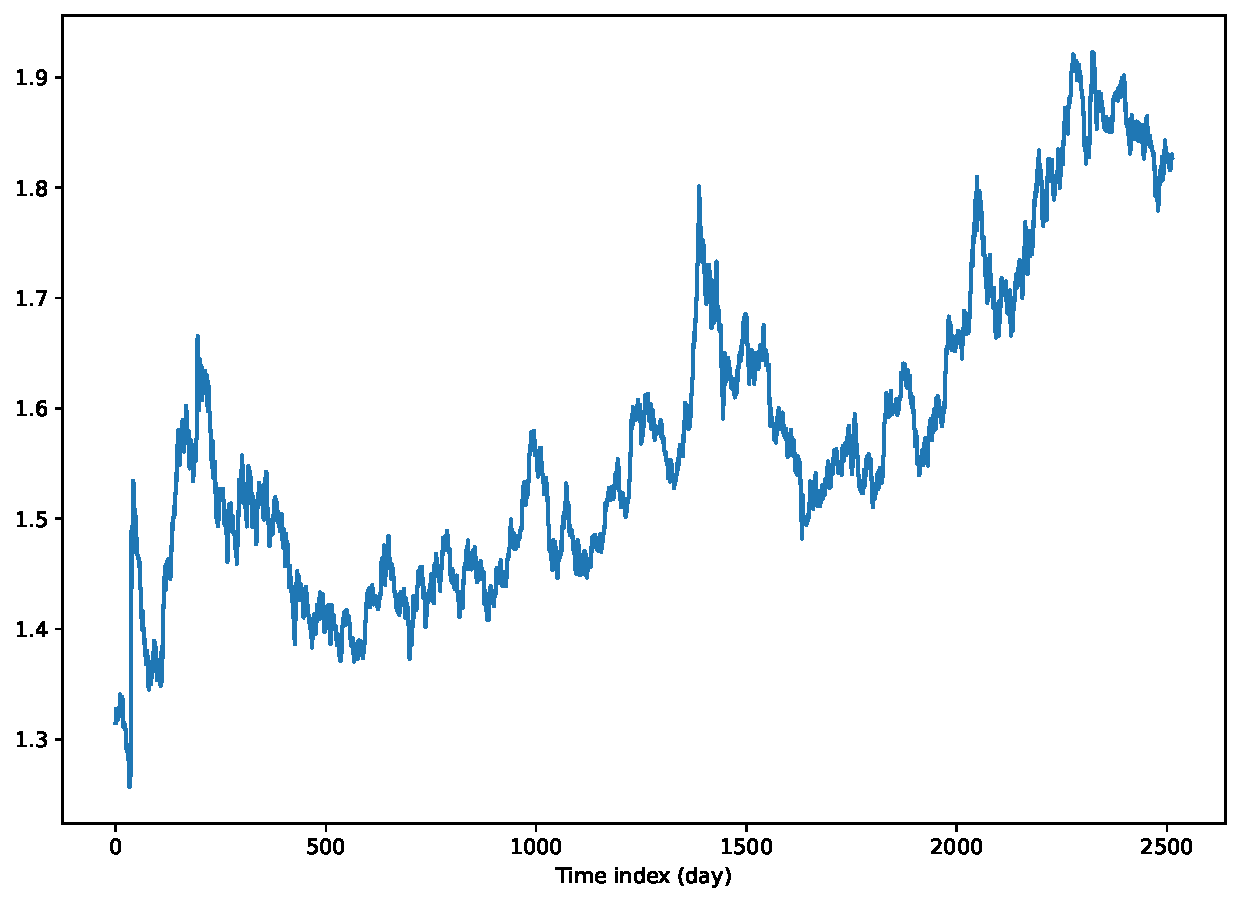
\includegraphics[width=\linewidth]{img/CHF_NZD.pdf}
    \caption{Exchange rate (close price) between Swiss franc and New Zealand dollar by day (2014-2024).}
    \label{fig:fx}
\end{figure}

%%%%%%%%%%%%%%%%%%%%%%%%%%%%%%%%%%%%%%%%%%%%%%%%%%%
\section{Methodology}
\label{sec.method}
%%%%%%%%%%%%%%%%%%%%%%%%%%%%%%%%%%%%%%%%%%%%%%%%%%%

% nói tổng quan ở đây, vẽ cái hình và bỏ vào
% Phương pháp của chúng tôi bao gồm hai phần chính hoạt động song song nhau: (1) - Feature extraction; (2) - Parameter synthesis. Tổng quan phương pháp được minh họa trong hình \ref{fig:flow}. Trong phần feature extraction, chúng tôi kết hợp hai loại đặc trưng từ mạng \verb|CNN| và \verb|LSTM|. Trong phần parameter synthesis, chúng tôi sử dụng \verb|MAML| để tổng hợp tham số của các mô hình. Với sự góp mặt của các đặc trưng \verb|LSTM| và \verb|CNN|, chúng tôi kỳ vọng sẽ rút trích được các đặc trưng ẩn trong dữ liệu aperiodic. Bằng việc sử dụng \verb|MAML| trong quá trình tổng hợp trọng số, phương pháp đề xuất được kỳ vọng là một giải pháp thay thế hợp lý và hiệu quả cho các mô hình ensemble truyền thống trong việc giảm thiểu tác động của sự biến thiên variance, tổng hợp hiệu quả các yếu tố ngoại lai, cũng như giữ được các hidden long-term dependency ẩn trong quá khứ.

Our method consists of two main parts that work in parallel: (1) - Feature extraction; (2) - Parameter synthesis. The overview of the method is illustrated in \ref{fig:flow}. In the feature extraction part, we combine two types of features from \verb|CNN| and \verb|LSTM| networks. In the parameter synthesis part, we use \verb|MAML| to synthesize the parameters of the models. Due to the contribution of \verb|LSTM| and \verb|CNN| features, we expect to effectively extract hidden features from aperiodic data. By using \verb|MAML| in the weight synthesis process, the proposed method is expected to be a reasonable and effective alternative to traditional ensemble models in minimizing the impact of variance variation, effectively synthesizing external factors, and preserving hidden long-term dependencies in the past.

\begin{figure*}[ht]
    \centering
    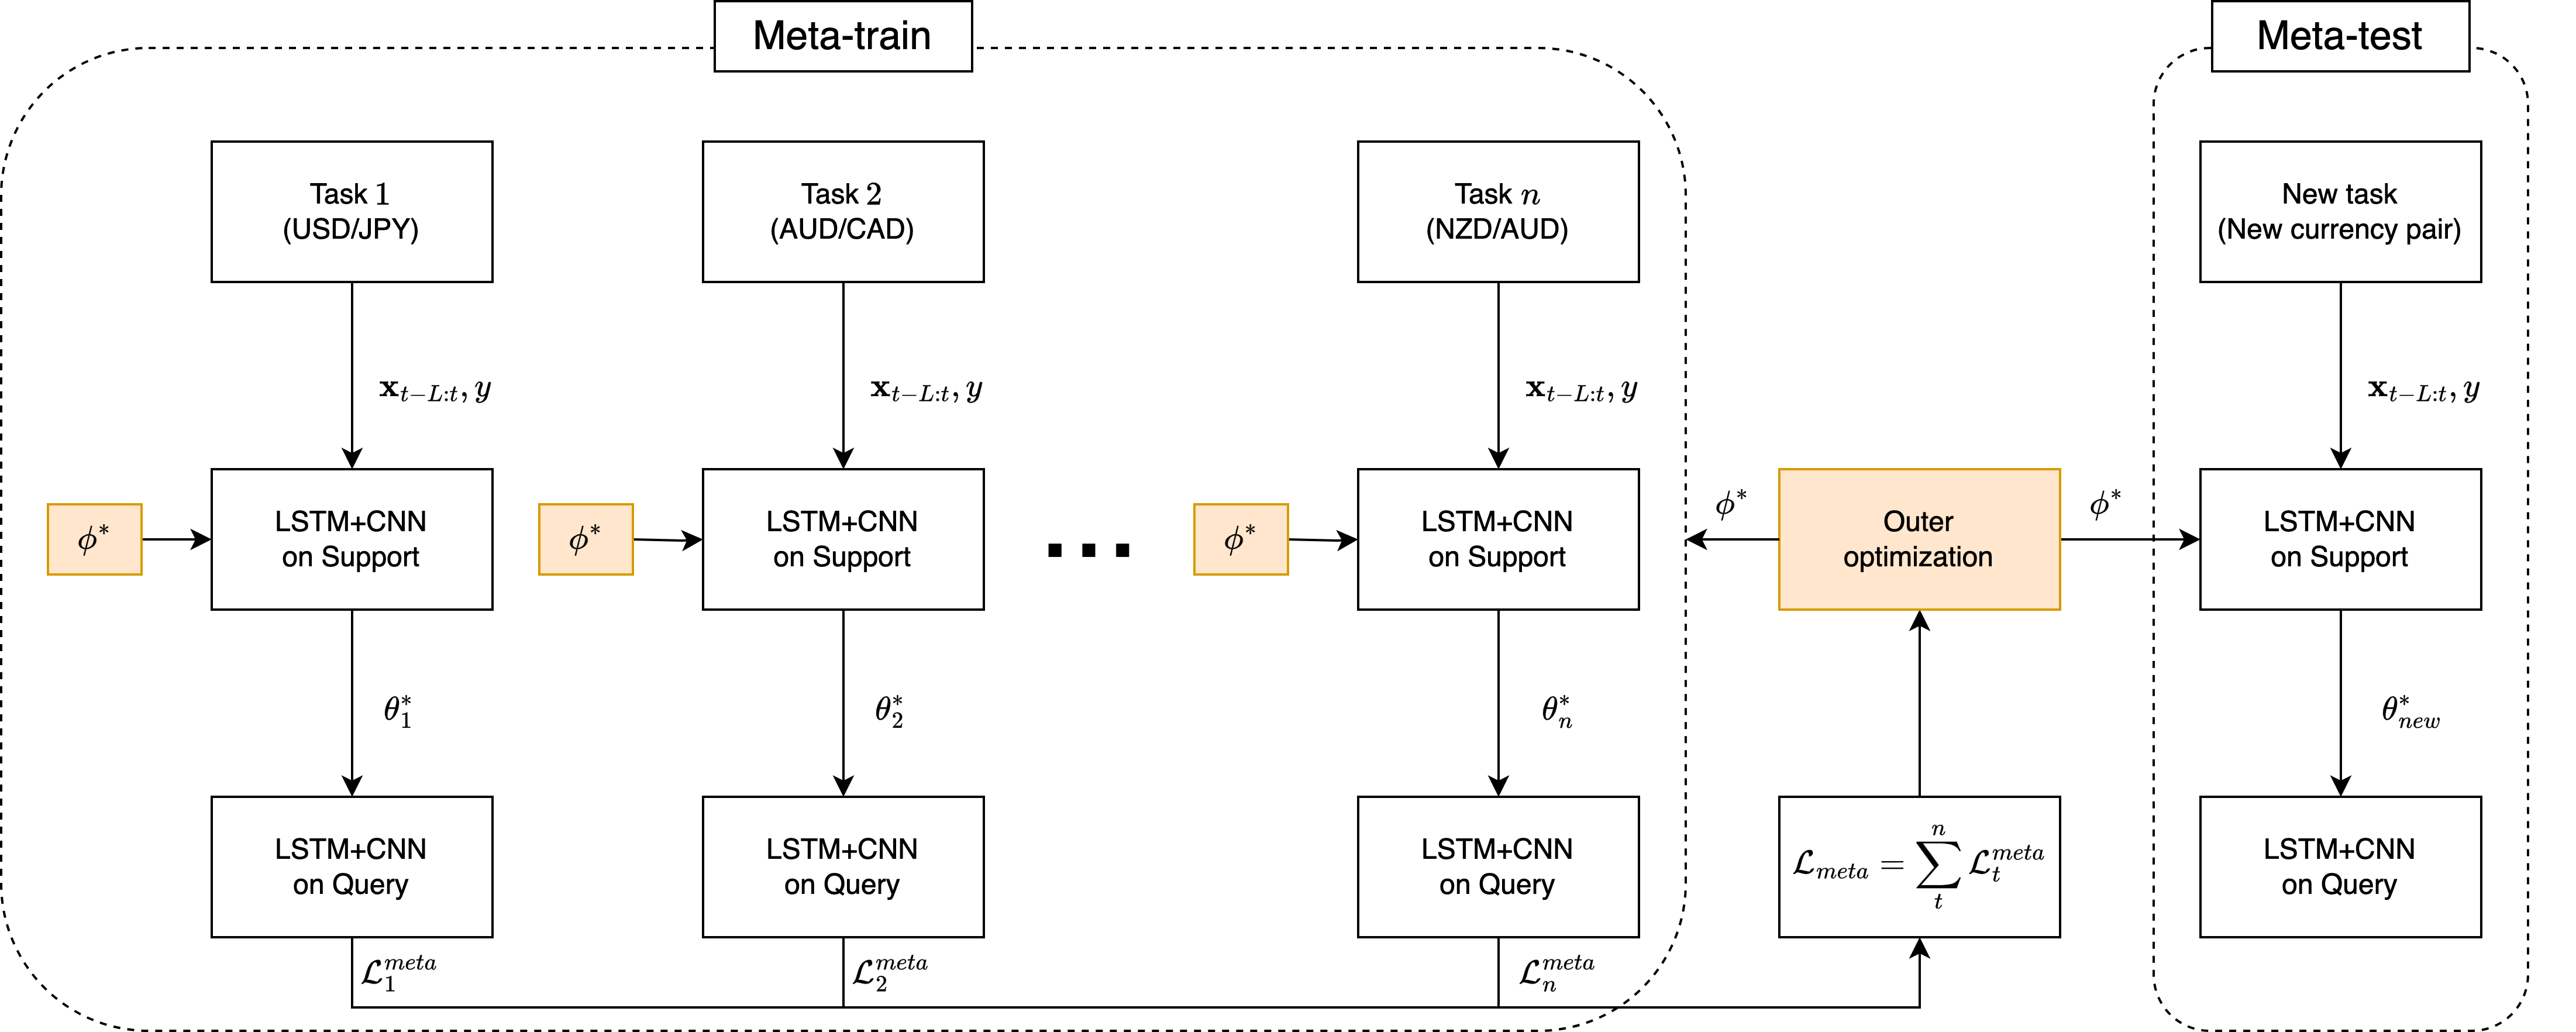
\includegraphics[width=\textwidth]{img/meta.png}
    \caption{The full-flow of meta-training and meta-testing on multi-fx data. Each currency pair is regarded as a task.}
    \label{fig:flow}
\end{figure*}

\subsection{Data preparation}

% Phương pháp đề xuất sử dụng các thuật toán ML để huấn luyện mô hình. Do đó, dữ liệu cần được tổ chức lại để các thuật toán ML có thể hoạt động được. Trong trường hợp dữ liệu bao gồm nhiều datasets khác nhau thuộc cùng một lĩnh vực, mỗi dataset sẽ được coi là một task của \verb|MAML|. Trong trường hợp dữ liệu bao gồm một dataset duy nhất, cần chia nhỏ dataset này thành các tập con ứng với các task riêng biệt. Tóm lại, tập dữ liệu sau khi chuẩn bị bao gồm $n$ tasks: $\mathcal{D} = \left\{ \mathcal{D}_t \right\}_{t=1}^{n}$. Dữ liệu tại mỗi task được chia thành tập support và query: $\mathcal{D}_t = \left\{ \mathcal{D}_t^{support}, \mathcal{D}_t^{query} \right\}$.

The proposed method uses ML algorithms to train the model. Therefore, the data needs to be reorganized so that the ML algorithms can work. In case the data includes many different datasets belonging to the same field, each dataset will be considered a task of \verb|MAML|. In case the data includes a single dataset, it is necessary to divide this dataset into subsets corresponding to separate tasks. In summary, the prepared dataset includes $n$ tasks: $\mathcal{D} = \left\{ \mathcal{D}_t \right\}_{t=1}^{n}$. The data at each task is divided into support and query sets: $\mathcal{D}_t = \left\{ \mathcal{D}_t^{support}, \mathcal{D}_t^{query} \right\}$.

\vspace{2mm}

% Một sample dữ liệu bao gồm các cặp giá trị $(\mathbf{x}_{t-L:t}, y)$. Trong đó, $\mathbf{x}_{t-L:t}$ bao gồm $L$ giá trị lịch sử tính từ thời điểm $t$ trở về trước; $y\in \{0,1\}$ là nhãn dữ liệu, thể hiện xu hướng giảm, hoặc tăng của mẫu dữ liệu $x_{t+1}$ so với $x_{t}$. Tùy vào từng bài toán và cách cài đặt mà các phần tử trong $\mathbf{x}_{t-L:t}$ có thể là các vector hoặc các scalar number. Ví dụ, đối với dữ liệu chứng khoán, $\mathbf{x}_{t-L:t}$ có thể chứa các vector dữ liệu $\vec x_i = (\text{open, low, high, close})$ hoặc chỉ một giá trị close price duy nhất.

A data sample consists of pairs of values $(\mathbf{x}_{t-L:t}, y)$. In which, $\mathbf{x}_{t-L:t}$ includes $L$ historical values from time $t$ back; $y\in \{0,1\}$ is the data label, showing the decreasing or increasing trend of the data sample $x_{t+1}$ compared to $x_{t}$. Depending on each problem and the implementation, the elements in $\mathbf{x}_{t-L:t}$ can be vectors or scalar numbers. For example, for stock data, $\mathbf{x}_{t-L:t}$ can contain $L$ data vectors $\vec x_i = (\text{open, low, high, close})$ or just a single close price value.

% nói từng cái, có thể sẽ vẽ hình cụ thể cho từng cái
% method phải chỉ ra được đoạn nào giải quyết thách thức nào (đã nêu ở intro)

% đến đoạn thực nghiệm thì sẽ mô tả sâu quá trình tìm kiếm tham số, quá trình chia dữ liệu, tải dữ liệu ở phụ lục
% nhận xét: nhấn mạnh vào việc giải quyết 3 thách thức nêu ở intro

\subsection{Feature extraction}

% Lấy cảm hứng từ nghiên cứu \cite{vo2017multi}, chúng tôi đề xuất kết hợp các đặc trưng rút trích được từ mạng \verb|LSTM| và \verb|CNN|. Cụ thể, chúng tôi đưa từng phần tử trong vector $\mathbf{x}_{t-L:t}$ qua một lớp \verb|MLP| có đầu ra lớn hơn số chiều của $\vec x_i, i\in[t-L, t]$ để phân giải thành các đặc trưng nhỏ $\vec x'_i$. Các đặc trưng này sau đó được truyền qua mạng \verb|LSTM| và \verb|CNN| để lần lượt rút trích các phụ thuộc thời gian dài hạn ($\mathbf{h}_{LSTM}$) và các đặc trưng thời gian cục bộ ($\mathbf{h}_{CNN}$). Để có thể khai thác tối đa các ràng buộc thời gian dài hạn, chúng tôi sử dụng \verb|BidirectionalLSTM| để rút trích từ hai phía của của $\mathbf{x}_{t-L:t}$. Toàn bộ quy trình rút trích đặc trưng được tóm tắt như sau:

Inspired by the \cite{vo2017multi} study, we propose to combine the features extracted from \verb|LSTM| and \verb|CNN| networks. Specifically, we pass each element in the vector $\mathbf{x}_{t-L:t}$ through a \verb|MLP| layer whose output'dimension is larger than the one of $\vec x_i, i\in[t-L, t]$ to decompose it into smaller features $\vec x'_i$. These features are then passed through \verb|LSTM| and \verb|CNN| networks to extract long-term temporal dependencies ($\mathbf{h}_{LSTM}$) and local temporal features ($\mathbf{h}_{CNN}$), respectively. To exploit the long-term temporal constraints, we use \verb|BidirectionalLSTM| to extract from both sides of $\mathbf{x}_{t-L:t}$. The entire feature extraction process is summarized as follows:

\begin{align}
    \mathbf{x'}_{t-L:t} &= \mathbf{FullyConnected}\left( \mathbf{x'}_{t-L:t} \right)\\
    \mathbf{h}_{LSTM} &= \mathbf{BidirectionalLSTM}\left( \mathbf{x'}_{t-L:t} \right)\\
    \mathbf{h}_{CNN} &= \mathbf{Convolution1D}\left( \mathbf{x'}_{t-L:t} \right)
    \label{eq:feature}
\end{align}

\vspace{2mm}

% Mạng \verb|LSTM| duy trì giá trị cell-state nhằm lưu trữ có chọn lọc các phụ thuộc dài hạn. Điều này rất thích hợp trong việc giải quyết các bài toán time-series data. Mặt khác, giá trị tương lai thường phụ thuộc rất lớn vào các giá trị lịch sử gần nhất. Chúng tôi đề xuất sử dụng mạng \verb|CNN| để nhấn mạnh các đặc trưng cục bộ, từ đó hướng một phần sự chú ý của mô hình vào các thời điểm nhất định. Do đó, phương pháp đề xuất không chỉ nhớ được các đặc trưng long-term mà còn highlight được các đặc trưng short-term.

The \verb|LSTM| network maintains cell-state values ​​to selectively store long-term dependencies. This is very suitable for solving time-series data problems. On the other hand, future values ​​often depend heavily on recent historical values. We propose to use the \verb|CNN| network to emphasize local features, thereby directing part of the model's attention to certain time points. Therefore, the proposed method can not only remember long-term features but also highlight short-term features.

\vspace{2mm}

% Tiếp đến, $\mathbf{h}_{LSTM}$ và $\mathbf{h}_{CNN}$ được nối với nhau (phương trình \ref{eq:concat}) sau đó chuyển đến phần phân lớp của mạng NN (phương trình \ref{eq:clf}).

Next, $\mathbf{h}_{LSTM}$ and $\mathbf{h}_{CNN}$ are concatenated (equation \ref{eq:concat}) and then passed to the classification part of the neural network (equation \ref{eq:clf}).

\begin{align}
    \mathbf{h}_{t-L:t} &= \mathbf{Concatenate}\left( \mathbf{h}_{LSTM}, \mathbf{h}_{CNN} \right) \label{eq:concat} \\
    \hat y &= \mathbf{FullyConnected}\left( \mathbf{h}_{t-L:t} \right) \label{eq:clf}
\end{align}

\subsection{Effective synthesis\\of models' parameters}

% Chúng tôi sử dụng \verb|MAML| để huấn luyện và tổng hợp trọng số của các mô hình tại các task. Như đã đề cập trong phần \ref{sec.relatedWork}, tối ưu tham số theo cách tiếp cận của ML chính là đi giải hai phương trình \ref{eq:inner_opt} và \ref{eq:outer_opt} bằng các phương pháp tối ưu trên dữ liệu support và query. Cụ thể, quá trình tối ưu bao gồm nhiều bước toàn cục (outer optimization), thực hiện trên tất cả các tasks tham gia huấn luyện. Mỗi bước toàn cục bao gồm nhiều bước cục bộ (inner optimization) thực hiện trên từng task riêng lẻ. Tại bước toàn cục $r$, quá trình tối ưu cục bộ lần thứ $e$ tại tập support của task $t$ diễn ra như sau:

We use \verb|MAML| to train and aggregate the weights of the models at the tasks. As mentioned in \ref{sec.relatedWork}, parameter optimization in the ML approach is to solve the two equations \ref{eq:inner_opt} and \ref{eq:outer_opt} using optimization methods on the support and query data. Specifically, the optimization process includes many global steps (outer optimization), performed on all tasks participating in training. Each global step includes many local steps (inner optimization) performed on each individual task. At global step $r$, the $e$th local optimization process at the support set of task $t$ occurs as follows:

\begin{align}
    \begin{cases}
        \theta_t^{(0)} &= \phi_{r-1} \\
        \theta_t^{(e)} &= \theta_t^{(e-1)} - \alpha \nabla_{\theta} \mathcal{L}^{task}_t\left( \theta_t^{(e-1)}, \mathcal{D}_t^{support} \right)
    \end{cases}
\end{align} In which, $\phi_{r-1}$ is the result of the $r-1$ global optimization process, $\alpha$ is the inner learning rate.

\vspace{2mm}

% Tiếp đó, quá trình outer optimization tại bước toàn cục được thực hiện bằng cách tổng hợp độ lỗi trên tập query của các task và tối ưu trên đó (phương trình \ref{eq:outer_sol}).

Next, the outer optimization process at the global step is performed by aggregating the losses on the query set of the tasks and optimizing on it (equation \ref{eq:outer_sol}).

\begin{align}
    \begin{cases}
        \phi_0 = \text{Random Initialization}\\
        \phi_r = \phi_{r-1} - \beta \nabla_{\phi} \sum_{t=1}^n{\mathcal{L}^{meta}_t \left( \theta_t^*(\phi), \mathcal{D}_t^{query} \right)}
    \end{cases}
    \label{eq:outer_sol}
\end{align} Where, $\beta$ is the outer learning rate.

% Giả sử thuật toán chạy $E$ steps trong inner optimization, lượng đạo hàm tại phương trình \ref{eq:outer_sol} được viết lại như sau (the notations of dataset are removed):

Assuming the algorithm runs $E$ steps in inner optimization, the derivative quantity at equation \ref{eq:outer_sol} is rewritten as follows (the notations of dataset are removed):

\begin{align*}
    &\beta \nabla_{\phi} \sum_{t=1}^n{\mathcal{L}^{meta}_t \left( \theta_t - \alpha \nabla_{\theta} \mathcal{L}^{task}_t\left( \theta_t \right) \right)}\\
    = &\beta \sum_{t=1}^n{ \frac{\partial \mathcal{L}^{meta}_t\left(\theta_t^{(E)}\right)}{\partial \theta_t^{(E)}} \frac{\partial \theta_t^{(E)}}{\partial \phi}}\\
    = &\beta \sum_{t=1}^n{ \nabla_{\theta} \mathcal{L}^{meta}_t\left(\theta_t^{(E)}\right) \prod_{j=0}^{E-1} {\left[\mathbb{I} - \alpha\nabla^2_{\theta}\mathcal{L}^{task}_{t}\left(\theta_t^{(j)}\right)\right]}} \numberthis
    \label{eq:outer_sol_}
\end{align*}

% Sự xuất hiện của tích các đạo hàm bậc hai trong phương trình \ref{eq:outer_sol_} khiến quá trình đạo hàm trở nên phức tạp vì phải tốn rất nhiều chi phí để duy trì các ma trận Hessian. Do đó, số bước tính toán để tìm ra $\theta^*$ cần phải hạn chế. Trên thực tế, các phương pháp sử dụng ML \citep{fallah2020personalized, chen2018federated, nguyen2022meta,finn2017model, li2017meta} thường sẽ chọn $E\in [1,5]$.

The presence of the product of second order derivatives in the equation \ref{eq:outer_sol_} makes the derivation process complicated because it requires a lot of overhead to maintain the Hessian matrices. Therefore, the number of computational steps to find $\theta^*$ needs to be limited. In practice, methods using ML \citep{fallah2020personalized, chen2018federated, nguyen2022meta,finn2017model, li2017meta} often choose $E\in [1,5]$.

%%%%%%%%%%%%%%%%%%%%%%%%%%%%%%%%%%%%%%%%%
\section{Numerical experiment}
\label{sec.experiment}
%%%%%%%%%%%%%%%%%%%%%%%%%%%%%%%%%%%e%%%%%%

\subsection{Dataset \& Metric}

% FX nói riêng và các chỉ số tài chính nói chung là dạng dữ liệu điển hình cho aperiodic time-series data. Do đó, chúng tôi chọn loại dữ liệu này để kiểm thử mô hình. Cụ thể, chúng tôi cấu hình hai bộ dữ liệu sử dụng dữ liệu FX. Bộ dữ liệu \verb|USD/JPY| chỉ gồm dữ liệu của cặp tiền tệ USD/JPY, được chia thành 60 tập dữ liệu con theo trình tự thời gian với kích thước bằng nhau. Dữ liệu được sample theo giờ từ năm 2000 đến năm 2024, bao gồm các thuộc tính open, low, high, và close price. Bộ dữ liệu \verb|multi-fx| bao gồm 60 cặp tiền tệ giữa 18 quốc gia Australia, Canada, Switzerland, Denmark, EU, United Kingdom, Hong Kong, Iceland, Japan, Norway, New Zealand, Singapore, Sweden, Turkey, United States, Mexico, China, South Africa. Dữ liệu có thuộc tính tương tự như \verb|USD/JPY| và được sample theo ngày từ năm 2014 đến 2024. Số lượng mẫu dữ liệu của hai tập dữ liệu là tương đương nhau và xấp xỉ $156000$ mẫu.

FX in particular and financial indices in general are typical data types for aperiodic time-series data. Therefore, we choose this type of data to test the model. Specifically, we configure two datasets using FX data. The \verb|USD/JPY| dataset consists of only data of the USD/JPY currency pair, divided into 60 time-sequenced subsets of equal size. The data is sampled hourly from 2000 to 2024, including the attributes of open, low, high, and close price. The \verb|multi-fx| dataset consists of 60 currency pairs made up of 18 countries: Australia, Canada, Switzerland, Denmark, EU, United Kingdom, Hong Kong, Iceland, Japan, Norway, New Zealand, Singapore, Sweden, Turkey, United States, Mexico, China, South Africa. The data has similar attributes to \verb|USD/JPY| and sampled daily from 2014 to 2024. The number of data samples of these two datasets are similar and approximately $156000$ samples.

\vspace{2mm}

% Bộ dữ liệu \verb|multi-fx| được sử dụng để rút trích và tổng hợp thông tin về các yếu tố ngoại lai (i.e. thông tin thị trường, kinh tế, chính trị,...), vốn được cho là có ảnh hưởng đến kết quả của một chỉ số tài chính nhất định \citep{overreactioncontrarian,fama1970efficient,mech1993portfolio}. Bộ dữ liệu \verb|USD/JPY| được sử dụng để kiếm chứng giả thuyết của chúng tôi về việc dữ liệu tương lai ngầm phụ thuộc vào các thời điểm nhất định trong quá khứ và cần phải tổng hợp đặc trưng quá khứ một cách hiệu quả để làm rõ được các phụ thuộc này.

The \verb|multi-fx| dataset is used to extract and aggregate information about outliers (i.e. market, economic, political, etc.) that are believed to influence the outcome of a given financial index \citep{overreactioncontrarian,fama1970efficient,mech1993portfolio}. The \verb|USD/JPY| dataset is used to test our hypothesis that future data implicitly depend on certain points in the past and that efficient past feature aggregation is needed to reveal these dependencies.

\vspace{2mm}

% Nghiên cứu sử dụng macro accuracy, macro precision, macro recall, và macro F1 để đánh giá các mô hình. Theo đó, trong quá trình inference, mô hình sẽ chạy trên từng task để tính metrics của mỗi task. Sau đó tính trung bình cộng các metrics của các task để thu được kết quả cuối.

The study uses macro accuracy, macro precision, macro recall, and macro F1 score to evaluate the models. Accordingly, during the inference phase, the model will run on each task to calculate the metrics of each task. Then, the average of the metrics of the tasks is calculated to obtain the final result.

\vspace{2mm}

\subsection{Experiment}

% Chúng tôi tiến hành so sánh phương pháp đề xuất với mô hình \verb|NHITS| thông qua các metrics nêu trên. Dữ liệu tổng quan được cấu trúc thành training sets, validation sets, và testing sets với tỷ lệ 6:2:2. Tập train dùng để huấn luyện mô hình, tập validation dùng để tìm kiếm siêu tham số và tập test để đánh giá mô hình. Đối với \verb|NHITS|, chúng tôi chia dữ liệu như bình thường theo tỷ lệ định sẵn ở trên. Đối với thuật toán đề xuất, vì quá trình meta-training và meta-testing đòi hỏi phải chia dữ liệu thành các task nhỏ, và cho phép mô hình adapt trên tập support của mỗi task, chúng tôi chia dữ liệu thành 60 tasks. Trong mỗi task, tập support chiếm 20\% với mục đích để mô hình học cách thích ứng với dữ liệu, tập query chiếm 80\% để kiểm tra khả năng tương thích của mô hình. Chúng tôi sử dụng 30 tasks để meta-train, 15 tasks để meta-validate, 15 tasks để meta-test. Với cách chia này, chúng tôi đảm bảo được tính công bằng khi mô hình ML được huấn luyện với lượng dữ liệu tương đương mô hình \verb|NHITS|.

We compare the proposed method with \verb|NHITS| using the above metrics. The overall data is structured into training sets, validation sets, and testing sets with a ratio of 6:2:2. The training set is used to train the model, the validation set is used to find hyper-parameters, and the test set is used to evaluate the model. For \verb|NHITS|, we split the data as usual according to the above predetermined ratio. For the proposed algorithm, because the meta-training and meta-testing processes require dividing the data into small tasks, and allowing the model to adapt on the support set of each task, we split the data into 60 tasks. In each task, the support set accounts for 20\% with the purpose of letting the model adapt to the data, the query set accounts for 80\% to check the model's compatibility. We use 30 tasks for meta-training, 15 tasks for meta-validation, and 15 tasks for meta-testing. With this division, we ensure the fairness that the ML model is trained with the same amount of data as \verb|NHITS|.

\vspace{2mm}

% Trong cài đặt của chúng tôi, chúng tôi sử dụng một lớp \verb|FullyConnected| gồm 16 units với hàm kích hoạt \verb|ReLU| để phân giải đặc trưng ban đầu. Sau đó, đặc trưng này được truyền song song đến các hai khối \verb|BidirectionalLSTM| và \verb|CNN|. Khối \verb|BidirectionalLSTM| bao gồm 32 hidden units, các đầu ra được nối dài để tạo thành một vector cuối. Khối \verb|CNN| bao gồm hai layer \verb|CNN| có số filter lần lượt là 32 và 64. Kernel được sử dụng trong các layer có kích thước $3\times 3$. Theo sau mỗi layer \verb|CNN| là một layer \verb|MaxPooling| sử dụng kernel kích thước $2\times 2$. Kết thúc khối \verb|CNN| là một layer \verb|Flatten|. Đặc trưng của khối \verb|BidirectionalLSTM| và \verb|CNN| sau đó được nối lại rồi truyền qua một layer phân lớp nhị phân với hàm kích hoạt \verb|Sigmoid|.

In our implementation, we use a \verb|FullyConnected| layer of 16 units with a \verb|ReLU| activation function to decompose the initial feature. This feature is then passed in parallel to the \verb|BidirectionalLSTM| and \verb|CNN| blocks. The \verb|BidirectionalLSTM| block consists of 32 hidden units, the outputs of which are concatenated to form a final vector. The \verb|CNN| block consists of two \verb|CNN| layers with 32 and 64 filters, respectively. The kernel used in the layers is of size $3\times 3$. Each \verb|CNN| layer is followed by a \verb|MaxPooling| layer using a kernel of size $2\times 2$. The \verb|CNN| block ends with a \verb|Flatten| layer. Features of the \verb|BidirectionalLSTM| and \verb|CNN| blocks are then concatenated and passed through a binary classification layer with a \verb|Sigmoid| activation function.

% Đối với mô hình \verb|NHITS|, chúng tôi sử dụng 

%%%%%%%%%%%%%%%%%%%%%%%%%%%%%%%%%%%%%%%%%%%%%%%%
\section{Results and discussion}
\label{sec.results}
%%%%%%%%%%%%%%%%%%%%%%%%%%%%%%%%%%%%%%%%%%%%%%%%



\begin{table*}[h]
    \centering
    \caption{Classification results (\%) of NHITS and our method using USD/JPY and multi-fx datasets. Best results per metrics are boldfaced.}
    \label{tab:rs}
    \begin{tabular}{c|c|cccc}
        \toprule
        \multicolumn{1}{c}{}        &       & $accuracy$ & $precision$ & $recall$ & $F1$  \\ 
        \hline
        \multirow{2}{*}{\Verb|USD/JPY|}    & \Verb|NHITS| & 53.29      & 52.38    & 52.23       & 51.87      \\
                                    & Ours  & $\mathbf{58.05±0.01}$ & $\mathbf{59.57±2.53}$ & $\mathbf{58.31±2.57}$ & $\mathbf{56.6±3.74}$    \\ 
        \hline
        \multirow{2}{*}{\Verb|multi-fx|} & \Verb|NHITS| & 51.12      & 51.22      & 51.16      & 50.54        \\
                                    & Ours  & $\mathbf{62.39±0.06}$ & $\mathbf{71.11±9.34}$ & $\mathbf{70.14±9.6}$  & $\mathbf{69.21±11.07}$  \\
        \bottomrule
    \end{tabular}
\end{table*}

% nói 1 chút về việc xài lstm+cnn/meta-learning sẽ giảm sự phụ thuộc của kết quả vào mạng NN/siêu tham số
% cụ thể, khi xài ML, tham số finetune rất dễ, cái nào cũng cao, chỉ cần chọn ra cái cao nhất
% giải thích tại sao cnn perform poorly: quá chú ý đến đặc trưng cục bộ mà quên mất các phụ thuộc dài hạn

%%%%%%%%%%%%%%%%%%%%%%%%%%%%%%%%%%%%%%%%%
\section{Conclusion \& Future direction}
\label{sec.conc}

% cite Meta-SGD, và 1 đống ML method vào đây để kiểu *ML có nhiều phương pháp, cần chạy thực nghiệm nhiều hơn
% cite iMAML, Reptile vào đây để làm future direction kiểu tối ưu lại ML vì chi phí hơi đắt

%%%%%%%%%%%%%%%%%%%%%%%%%%%%%%%%%%%%%%%%%

% Conclusion

%%%%%%%%%%%%%%%%%%%%%%%%%%%%%%%%%%%%%%%%%
\section{Acknowledgements}
%%%%%%%%%%%%%%%%%%%%%%%%%%%%%%%%%%%%%%%%%
% The work was carried out within the state assignment of Ministry of Science and Higher Education of the Russian Federation (No. AAAA-A18-118020190095-4, topic ``Quantum''). G.I.P is grateful for financial supports from JST SPRING, Grant Number JPMJSP2102. K. H. is grateful for financial support from MEXT-KAKENHI (JP19K05029, JP21K03400, JP21H01998, and JP22H02170). R.M. is grateful for financial supports from MEXT-KAKENHI (22H05146, 21K03400 and 19H04692).

%%%%%%%%%%%%%%%%%%%%%%%%%%%%%%%%%%%%%%%%%
\section{Author contributions}
%%%%%%%%%%%%%%%%%%%%%%%%%%%%%%%%%%%%%%%%%
% All authors contributed to conceiving the idea. T.I., A.V.U, and G.I.P performed the calculations. T.I. made the all figures. R.M and S.V.S supervised the work. All authors contributed to the discussion and writing of the paper.

%%%%%%%%%%%%%%%%%%%%%%%%%%%%%%%%%%%%%%%%%
\section{Data availability statement}
%%%%%%%%%%%%%%%%%%%%%%%%%%%%%%%%%%%%%%%%%
% The datasets used and/or analyzed during the current study available from the corresponding authors on reasonable request.

%%%%%%%%%%%%%%%%%%%%%%%%%%%%%%%%%%%%%%%%%
\bibliographystyle{elsarticle-harv} 
\bibliography{references}
\end{document}
%%%%%%%%%%%%%%%%%%%%%%%%%%%%%%%%%%%%%%%%%



%%%%%%%%%%%%%%%%%%%%%%%%%%%%%%%%%%%%%%%%%%
%\section{Appendix}
%%%%%%%%%%%%%%%%%%%%%%%%%%%%%%%%%%%%%%%%%%
%We used the VASP code\cite{VASP} for the calculations explained in this appendix.
%We relaxed the four structures of Figure \ref{fig.str}
%for every LiV$X_2$ ($X$ = O, S, and Se) with each of PBE\cite{PBE},
%optPBE-vdW-DF\cite{2009JK_AM,vdW-DFa,vdW-DFb}, and HSE06\cite{HSE06} functionals.
%We evaluated the relative energies of structures relaxed by every functional by PBE-DFT.
%%as shown in Figure \ref{fig.geomErr}.
%We found that the differences of the relative energies
%among the structures relaxed by different functionals are at most 0.018 eV/f.u.
%%the differences of the time-series in Figure \ref{fig.geomErr} are within 0.018 eV/f.u.

%%----------------------------------------
%\begin{figure}[htbp]
%  \centering
%  \includegraphics[width=\hsize]{geomErr.eps}
%  \caption{\ghost{fig.geomErr}\label{fig.geomErr}
%    FNDMC and DFT results of relative energies of the four candidate structures
%    of LiV$X_2$ (X = O, S, and Se).
%    The candidate structures are shown in Figure \ref{fig.str}.
%    TR-I and TR-II (left from the vertical line) are trimmerized
%    and NTR-I and NTR-II (right from the vertical line) are
%    non-trimmerized structures, respectively.
%    FNDMC results are same as Figure \ref{fig.dmconly}.
%    The lowest energy among the four structures is set to be zero
%    and the others are given as relative values from the lowest energy.
%  }
%\end{figure}
%%----------------------------------------
